\documentclass[aspectratio=169]{beamer}
%\documentclass{beamer}
% changed aspect ratio to 16:9 to match the background image; still works even if this is removed
\setbeamertemplate{navigation symbols}{}
\setbeamercolor{frametitle}{fg=red}
\setbeamercolor{title}{fg=white}
\setbeamercolor{author}{fg=white}
\setbeamercolor{date}{fg=white}
\setbeamerfont{frametitle}{family=\rmfamily,shape=\itshape,size=\huge} 
\setbeamerfont{title}{family=\rmfamily,shape=\itshape,size=\huge} 
\usetheme{boxes}
\setbeamertemplate{footline}[frame number]
\setbeamertemplate{itemize/enumerate body begin}{\small}
\setbeamertemplate{itemize/enumerate subbody begin}{\footnotesize}


\newcommand{\mcal}{\textsc{metacalibration}}
\newcommand{\Mcal}{\textsc{Metacalibration}}
\newcommand{\ngmix}{\texttt{ngmix}}
\newcommand{\imshape}{\textsc{im3shape}}

\newcommand{\bdkfull}{Bulge+Disk+Knots}
\newcommand{\bdksim}{\texttt{BDK}}
\newcommand{\bdstar}{\texttt{BDK+Stars}}
\newcommand{\bdmask}{\texttt{Mask}}
\newcommand{\rgsim}{\texttt{RG}}
\newcommand{\pimprovement}{90}

\newcommand{\snr}{$S/N$}

%
%Global Background must be put in preamble
%-rescale the 16:9 image to slide size choice
\usebackgroundtemplate{
\includegraphics[width=\paperwidth,height=\paperheight]{bnl_interior}}
%
\title{Erin Sheldon's Roles in DES and LSST}
\author{Erin Sheldon}
\date{July 10, 2019}
%
\begin{document}
{\usebackgroundtemplate{
\includegraphics[width=\paperwidth,height=\paperheight]{bnl_title}}
\maketitle
}


%
\frame
{

    \frametitle{Erin Sheldon's Role in DES}

    %\setbeamerfont*{itemize/enumerate body}{size=\large}

    \begin{columns}
        \begin{column}{0.5\textwidth}
            \centering
                \includegraphics[height=0.8\textheight]{ctio_blanco_crew_2013Oct-30-small-balance.jpg}
                \newline
                {\tiny Image Brian Nord}
        \end{column}

        \begin{column}{0.5\textwidth}
            \begin{itemize}

                \item Erin Sheldon is responsible for the primary measurements
                    of objects in the survey

                \item Brightness, size, shape of stars and galaxies.

                \item Responsible for the all of the basic weak lensing measurements
                    for each object in the survey.

                \item Finishing up work for Year 3, beginning work or the final Year 6 data set.

                \item In the critical path for all key projects other than supernovae.

            \end{itemize}

        \end{column}

    \end{columns}


}

\frame
{

    \frametitle{Erin Sheldon's Role in LSST}

    %\setbeamerfont*{itemize/enumerate body}{size=\large}

    \begin{columns}

        \begin{column}{0.5\textwidth}
            \begin{itemize}

                \item Responsible for the basic weak lensing measurements for
                    each object in the survey.

                \item Has integrated the basic code into the measurement framework.

                \item The code is being run on the simulation data challenge (DC2).

                \item Developing a more accurate version of the algorithm needed
                    for LSST, nearly complete.

            \end{itemize}

        \end{column}

        \begin{column}{0.5\textwidth}
            \centering
                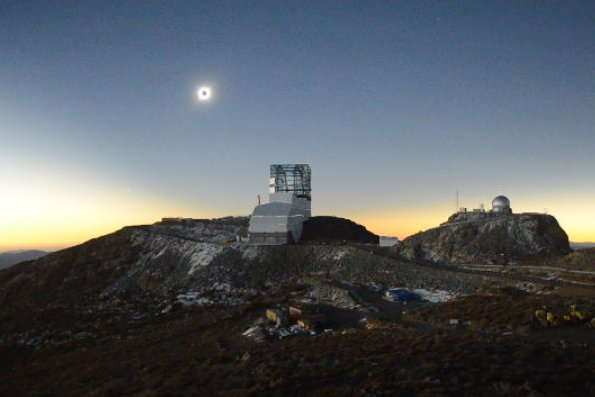
\includegraphics[height=0.8\textheight]{LSST-eclipse-2019.jpg}
                \newline
                {\tiny 2019 Eclipse with Earth Cam}
        \end{column}

    \end{columns}


}




\end{document}
